%&xelatex


% Edit links (please keep save: https://www.overleaf.com/3988312979bwydrcpjsrht#f1fe60)
% Read link: https://www.overleaf.com/read/frscmwxxqhcq#edf650

%%%%%%%%%%%%%%%%%%%%%%%%%%%%%%%%%%%%%%%%%%%%%%%%%%%%%%%%%%%%%%
%%%%%%%%%%%%%%%%%%%%%%% README %%%%%%%%%%%%%%%%%%%%%%%%%%%%%%%
%%%%%%%%%%%%%%%%%%%%%%%%%%%%%%%%%%%%%%%%%%%%%%%%%%%%%%%%%%%%%%

%% Information for colleagues accessing this document, such as Russell (G), Russell (B), Stephen, Angela, Simon, Mary etc.

%% If you have the time and feel generous, you are welcome to read through and give comments on this document.

%% The comment character in Latex is "%". Any line that starts with % will not be rendered in the document. So, you can add text in this way and you can ignore any text that I or someone else have commented out. Overleaf will render this text in green in the Code Editor.

%% Thank you for your time, knowledge and patience.

%%%%%%%%%%%%%%%%%%%%%% HOW TO COMMENT %%%%%%%%%%%%%%%%%%%%%%%%
%% Here are instructions for how to add a comment in Overleaf's online collaborative interface: https://www.overleaf.com/learn/how-to/How_to_make_comments_in_an_Overleaf_LaTeX_project#Commenting:_feature_overview

%% If you wish to leave comments directly in the LaTeX code, you can. Please start such comments with %#comment #STEPHEN (or other name). That way I can easily find them and know who has written what.

%% Instructions for downloading PDF: https://www.overleaf.com/learn/how-to/Exporting_your_work_from_Overleaf#Downloading_the_typeset_PDF_file

%% If you download the document as a PDF and make comments that way, the easiest on my end is if you write comments in a txt-file or Preview. If you use a PDF annotation, if you could please use Preview because other programs tend to crash or otherwise cause problems I am afraid. 

%% AGAIN: THANK YOU :D

%%%%%%%%%%%%%%%%%%%%%%%%%%%%%%%%%%%%%%%%%%%%%%%%%%%%%%%%%%%%%%
%%%%%%%%%%%%%%%%%%%%%%%%%%%%%%%%%%%%%%%%%%%%%%%%%%%%%%%%%%%%%%
%%%%%%%%%%%%%%%%%%%%%%%%%%%%%%%%%%%%%%%%%%%%%%%%%%%%%%%%%%%%%%

%\documentclass[12pt,letterpaper]{article}
\documentclass[unnumsec,webpdf,modern,medium]{oup-authoring-template}

%\usepackage[lmargin=1.2in,rmargin=1.2in,tmargin=1in,bmargin=1in]{geometry}
%\usepackage[bf,tiny]{titlesec}
%\usepackage{fontspec,xltxtra,xunicode}
    	%\defaultfontfeatures{Mapping=tex-text}
%\usepackage[utf8]{inputenc}
%\usepackage[utf8]{fontenc}
%\setmainfont{Junicode}

\usepackage{setspace}
%\usepackage{gb4e}
%\let\eachwordone=\it %italicise the first line of examples
%\usepackage[sort]{natbib}
%\bibpunct[: ]{(}{)}{,}{a}{}{,}
%\usepackage{afterpage}
%\usepackage{graphicx}
% OUP PACKAGES
%\graphicspath{{Fig/}}

% line numbers
\usepackage{lineno}
\linenumbers

% extra packages beyond OUP
\usepackage{placeins} %to enable float barriers
%\usepackage{CJKutf8} %chinese caracthers
%\usepackage{amsmath} % for equations
\usepackage{graphicx} 
\usepackage{booktabs} % for nice looking tables
\usepackage{longtable} %for tables stretching several pages
\usepackage{pdflscape} %for making things landscape
%\usepackage{multirow} %merging rows in tables
%\usepackage{caption} %for making subfigures
%setting a float environment for lists
%\usepackage{enumitem} %make it possible to have other enumerate items, like roman numerals
\usepackage[english]{babel} % To obtain English text with the blindtext package
\usepackage{blindtext}

\usepackage{colortbl}
\definecolor{spec_color_lightgreen}{HTML}{81F093}
\definecolor{spec_color_lightgrey}{HTML}{e6e6e6}



%\usepackage{authblk}
%\usepackage{draftwatermark}
%\SetWatermarkText{DRAFT}
%\SetWatermarkScale{4}

%\pagestyle{myheadings}


%\author{anon}

%\setlength{\parindent}{0pt}
%\setlength{\parskip}{1ex plus 0.5ex minus 0.2ex}

\usepackage{xr-hyper}%for referenxing appendecies
\usepackage{hyperref}

\makeatletter
\newcommand*{\addFileDependency}[1]{% argument=file name and extension
\typeout{(#1)}% latexmk will find this if $recorder=0
% however, in that case, it will ignore #1 if it is a .aux or 
% .pdf file etc and it exists! If it doesn't exist, it will appear 
% in the list of dependents regardless)
%
% Write the following if you want it to appear in \listfiles 
% --- although not really necessary and latexmk doesn't use this
%
\@addtofilelist{#1}
%
% latexmk will find this message if #1 doesn't exist (yet)
\IfFileExists{#1}{}{\typeout{No file #1.}}
}\makeatother

\newcommand*{\myexternaldocument}[1]{%
\externaldocument{#1}%
\addFileDependency{#1.tex}%
\addFileDependency{#1.aux}%
}

\myexternaldocument{appendices}




\begin{document}

\journaltitle{Journal of Language Evolution}
\DOI{N/A}
\copyrightyear{N/A}
\pubyear{N/A}
\access{Advance Access Publication Date: N/A}
\appnotes{Paper}

\firstpage{1}

%\subtitle{Subject Section}

\title[Predicting number of languages in Remote Oceania]{A Sea of Languages: predicting the number of languages per island group in Remote Oceania}

%\author[1,$\ast$]{Hedvig Skirgård}
\author[1,$\ast$]{Anonymous Author}

\authormark{ANON}

%\address[1]{\orgdiv{Department of Linguistic and Cultural Evolution}, \orgname{Max Planck Institute for Evolutionary Anthropology}, \orgaddress{\street{Deutscher Platz 6}, \postcode{04103}, \state{Saxony}, \country{Germany}}}

\address[1]{\orgdiv{Department}, \orgname{Organization}, \orgaddress{\street{Street}, \postcode{Postcode}, \state{State}, \country{Country}}}

\corresp[$\ast$]{Corresponding author. }
%\corresp[$\ast$]{Corresponding author. \href{email:Hedvig_skirgard@eva.mpg.de}{Hedvig\_skirgard@eva.mpg.de}; +46 72 853 96 73}


\received{Date}{0}{Year}
\revised{Date}{0}{Year}
\accepted{Date}{0}{Year}

%\editor{Associate Editor: Name}

%\abstract{
%\textbf{Motivation:} .\\
%\textbf{Results:} .\\
%\textbf{Availability:} .\\
%\textbf{Contact:} \href{name@email.com}{name@email.com}\\
%\textbf{Supplementary information:} Supplementary data are available at \textit{Journal Name}
%online.}
%We suggest a maximum length of 350 words for the Abstract

\abstract{There are more than 7,000 languages on our planet today, but they are not evenly distributed. There are over 100 languages in Vanuatu, but only one in S\={a}moa. This is in spite of the populations being similarly sized, having similar histories etc. Why might this be? This paper explores this question for one particular region: Remote Oceania. Remote Oceania comprises the eastern Solomon Islands (Temotu), Vanuatu, New Caledonia, Fiji, Polynesia and Micronesia. The region was settled more recently than the rest of Oceania and initially entirely by Austronesian speakers. Through studies in archaeology, history and linguistics, as well as community knowledge, much is known about migration patterns and societal organization of this part of the world. The comparatively shallow time depth, the relatedness of the languages and established knowledge about the history make it an ideal base for understanding language diversification. One particular theory has been proposed to explain the discrepancy in language richness over Remote Oceania --- societal organisation. In this study, we test if this factor remains an important predictor of the number of languages also when other relevant factors are taken into account, such as time-depth and environment, using a Bayesian Regression model approach. The results show that the theory does hold in terms of statistical power, but that there are important caveats such as the instantiation of the variable ``political complexity'' and its relationship with contact with Oceanic neighbours in the New Guinea region.}

%Scholars have suggested several reasons for the large discrepancy between the number of languages per island group in Remote Oceania, such as societal organisation, environmental factors and settlement time. 


\keywords{languages, Oceania, predicting, political complexity}

\maketitle

\newpage

%%toberemoved %\doublespacing


\onecolumn
\section{Introduction}
\doublespacing

The number of languages in the world is not equally distributed over area and population. In the modern country of Papua New Guinea, there are 835 languages over a population of 9.7 million people \citep{UN_pop, glottolog3}. However, in South Korea, there are only two indigenous spoken languages in a population of 52 million people. How can this be?

Understanding the mechanics of language change and diversification is essential to understanding human history. Language is interlinked with cultural identity, learning about the historical dynamics of language informs our understanding of our story generally. The question of language splitting in particular is interesting as it also implies community splitting. What causes us to lose touch, to diverge and go separate ways? This research topic has received a lot of attention in recent years (cf. \citet{gavin2017process,  greenhill2015demographic, Pacheco_Coelho_2019, hua2019ecological}). In this study, we will take a closer look specifically at the region of Remote Oceania. 

Fig.~\ref{RO_overnight_coloured_dots} shows the language richness of the islands of Oceania. Languages are points, coloured by language family. In the Polynesian islands (S\={a}moa, Tonga, Rarotonga, Tokelau etc), there is generally one language per island group. However, in central west Remote Oceania (Vanuatu, Temotu, Fiji and Kanaky) there are many more languages --- sometimes up to 20 languages on the very same island. The archipelagos of Chuuk, Wa'ab and Pohnpei also feature more languages than the Polynesian islands and atolls. What explains this difference?
%What are the mechanics of this?

\begin{sidewaysfigure}[p]
\centering
\includegraphics[width=\textwidth]{CartoGIS_oceania_languages_subgreions_edited}
\caption{Map of Oceania, with the regions of Near and Remote Oceania marked out (first labelled by \citet{pawley1973dating}). Points represent languages, based on data \citet{glottolog3} with a few small adjustments by author.} 
\label{RO_overnight_coloured_dots}
\end{sidewaysfigure}

Let us first consider some plausible factors in language diversification. Firstly, diversification takes time. We would expect a higher probability of language diversification in areas where people have lived for a longer time simply due to natural drift as communities spread out and form separate clusters. All of Remote Oceania was settled in approximately the last 3,500 years but at different stages. A large part of Remote Oceania was settled for the first time by Austronesian-speaking people in a rapid expansion 3,600 - 2,800 BP known as the ``Lapita expansion'' (\citet[106-7]{bellwood2006austronesians}; \citet[137]{rieth_cochrane_2018}). This first area covers all islands of Vanuatu, Temotu, New Caledonia, Fiji and parts of Western Polynesia. The dates of the first settlement for these islands are relatively similar, but there still is a large discrepancy in the number of languages (see Fig \ref{RO_overnight_coloured_dots}). This makes for a convenient case for comparison. If we include other regions of Oceania, such as Australia or the New Guinea region \citep{ross2017_new_guinea_region}, the comparison becomes more complex as they have been settled for a much much longer time-span --- possibly up to 60,000 years. Here we focus specifically on Remote Oceania in order to test specific theories about the diversification there that have been presented by anthropologists and linguists.

Let us compare two island groups in this region as an example: the S\={a}moan archipelago in Western Polynesia and the island of Malakula in Vanuatu. There is one indigenous language spoken in S\={a}moa ---  S\={a}moan --- and in Malakula there are 33 distinct languages spoken \citep{glottolog3}. S\={a}moa was settled approximately 400 years after Malakula \citep[137-8]{rieth_cochrane_2018}. This gives Malakula a bit of a ``head-start'', but most likely not enough to explain the vast difference.

Besides time depth, we might also expect that more space entails greater language diversity. A larger area makes it possible to spread out communities, which can entail language splitting. However, the shoreline\footnote{Since Austronesian settlements are mainly found on the coast, we are comparing shorelines instead of land area.} of Malakula is 67\% of that of S\={a}moa. S\={a}moa is larger than Malakula. What other factors are there that can aid our understanding here?

\citet{turner1884} and \citet{pawley81,pawley2007} have suggested that the discrepancy between the number of languages in different parts of Remote Oceania can be related to societal structure. Societies in Vanuatu and New Caledonia tend to be less hierarchical than societies in Polynesia. Societies with fewer vertical levels of political structure are associated with more linguistic and cultural diversity. Conversely, more hierarchically complex societies are associated with linguistic and cultural homogeneity.

%A measurement of so-called ``political complexity'' in ethnographic surveys (cf. \citet{gray1998ethnographic}) should then be correlated with different patterns of interaction and show up as a significant factor in language diversification. This is true even if political complexity is merely a proxy measurement of the interaction pattern that is in fact driving language change. 

This study tests the hypothesis that more vertical levels of political organisation are meaningfully connected to the number of languages, also when we incorporate other possible factors like settlement time, size and ecological environment (cf. \citet{NETTLE1998}, \citet{gavin2012island} and \citet{hua2019ecological}). If the results show that political complexity has a significant correlation with the number of languages per island group when other relevant factors are controlled for, this lends support to Turner and Pawley's hypothesis.
 
%We will be using cultural data on societal structures in societies of Remote Oceania, archaeological dates and environmental variables (temperature and rainfall) to test if the political structure still significantly predicts the number of languages once other factors have been taken into account. Fig.~\ref{RO_overnight_coloured_dots} shows languages in Oceania, with islands grouped by overnight sailing distances \citep{mark_1986, marck2000}. In this study, we are concerned with languages of Remote Oceania (see Fig.~\ref{Remote_Oceania_subregions} for subregions of Oceania), and in particular Vanuatu and New Caledonia compared to the rest.

%First, we will go through previous research, secondly, we will have an overview of the region given the variables we are using in the study. Thirdly, the method will be presented and lastly we will go through the results and possible interpretations of them.

\FloatBarrier
\section{Previous research}
\label{sec:previous_research}
Linguists, anthropologists and scholars of other fields have long remarked on the link between linguistic diversity and political structure in Remote Oceania. One of the oldest examples of this observation is the European Turner who travelled in the region 1861-1884 and hypothesized that the lack of regional variation \emph{within} S\={a}moan entailed that they had long had a centralized government \citep[172]{turner1884}. Linguists have linked types of societal organization to different diversification processes. Language change is embedded in social structure (cf. \citep{WLH1968}), or as \citet[124]{grace_1992_aberrant} writes: ``linguistic similarities and differences [are] reflections of community structures''. As community ties weaken and what was once one social network splits up, we expect that this is reflected in language variation as well. In this way, language studies provide insights to neighbouring fields such as archaeology, anthropology etc.

\citet{pawley81, pawley2007} discusses the specific hypothesis that while much of Remote Oceania was settled in similar ways by Austronesian-speaking people, and at comparable time depths, and developed similarly immediately after the first settlement, the differences between them stem from the rise of powerful chiefs and maintenance of long-distance voyaging in the island groups of Polynesia. This theory suggests that the steps of the diversification process were more or less the same, but that the \emph{rate} by which it progressed differed and that this is the cause for the variation we see today.\footnote{\citet{lynch1981melanesian} calls this ``the diversification cycle theory''.} 

%The societal structure in Polynesia was such that the process of cultural diversification was slower than in Vanuatu and New Caledonia. 

%The following quote from \citet{pawley2007} summarises a few of these points and links them to the political organisation:

%This diversification process has two stages. First, there are similar sequences of rapid expansion over the entire island group, and sparse settlement with trade and marriages between different sister communities. Second, there is denser settlement associated with localised trade and marriage practices between sister communities, more intensive agriculture and weakening of kin ties and linguistic divergence. 

%\begin{quotation}
%\noindent \emph{When they found a new island group the Lapita colonists rapidly explored and lightly settled it. This initial colonising phase was typically followed by a sequence of demographic, economic and technological developments. Population growth led to a denser distribution of settlements, more intensive agriculture, more local marriage and trade, weakening of kin ties with distant communities, and linguistic divergence. This sequence of events happened in both Southern Melanesia and West Polynesia and Fiji but it happened more slowly in West Polynesia/Fiji. In [Fiji and West Polynesia] the maintenance of long-distance voyaging, both within island groups and between neighbouring island groups, can be attributed in large part to the rise of powerful chiefs. These chiefs had political, economic and social motives for maintaining long distance connections and were able to use their authority to drive the production of a food surplus which in turn could be used to support specialist craftsmen who could, among other things, build and sail large ocean-going canoes.} \citep[28]{pawley2007} \end{quotation}

The hypothesis of \citet{pawley81, pawley2007} can be expressed in a Directed Acyclic Graph (DAG, cf. \citet{pearl1995causal} and \citet{mcelreath2020statistical}). This lets us view the chain of argumentation in a stylized and formal visualisation that can lead directly to statistical modelling and comparison between proposals (cf. \citet{roberts2020chield}). Fig. \ref{Predicting_lgs_DAG_andy} contains such a graph, based on the author's interpretation of Pawley's proposal in more detail. The connection between the rise of powerful chiefs and language richness is not direct, but mediated through a number of other factors. 

\begin{figure}[ht]
\centering
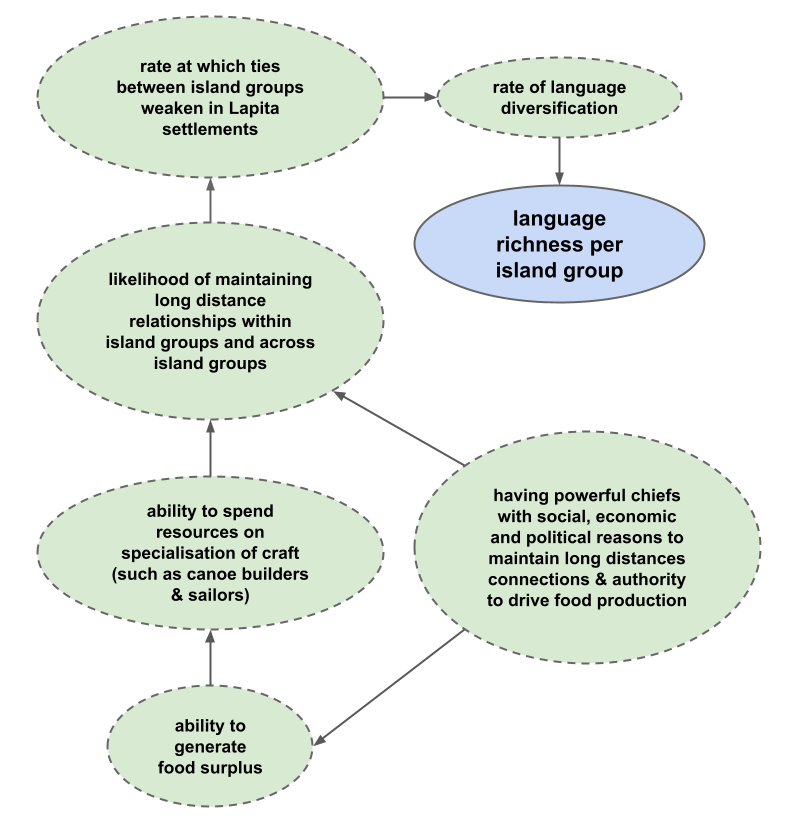
\includegraphics[width=0.5\textwidth]{Predicting_lgs_DAG_andy}
\caption{Directed Acyclic Graph of the argument presented in \cite{pawley2007}. Blue = variable to be predicted (response).}
\label{Predicting_lgs_DAG_andy}
\end{figure}

While political complexity may be a predictor of the number of languages, it is unlikely that this is directly due to individual powerful leaders having a direct effect on the nature of the language of the community by means of their personality, conscious policies or directives. It is possible the political structure is instead indicative of a certain community network structure and attitude. Fig. \ref{appendix_Predicting_lgs_DAG_full} in Appendix \ref{appendix_DAG_def} contains a larger version that incorporates more of the suggested linkages beyond those suggested by Pawley, for example, that political complexity may affect the modularity and interconnectedness of social networks and this, in turn, affects language splitting. 

In a similar vein to Pawley, \citet{curriemace2009} suggests that more stratified societies are correlated with larger language areas in Africa and Eurasia. If one language covers a large area, then the number of languages per square kilometre is lower than otherwise --- the language density is lower. Their research can be interpreted to mean that more stratified societal structures are more capable of sustaining linguistic homogeneity over a larger geographical area (or possibly reducing diversity by cultural dominance and warfare). Greater maintenance of cultural homogeneity would result in less language splitting over larger areas, and therefore a larger language area correlates with greater stratification. The approach is different from \citet{pawley81, pawley2007}, but the scientific line of argumentation is similar.


Returning to language richness in Remote Oceania, a significant factor to consider besides those already discussed is contact --- in particular with people from the New Guinea region (cf. \citet{ross2017_new_guinea_region}). Prior to European colonisation, all indigenous communities of Remote Oceania spoke the languages of the Austronesian family (see Fig \ref{RO_overnight_coloured_dots}). This family has its ultimate origins in Taiwan, and spread into the Remote Oceania approximately 3-4,000 years ago (cf. Fig. \ref{austro_expansion_bellwood}). The peopling of New Guinea, the Bismarck archipelago and much of the Solomon Islands however is older than that, and there is a great amount of language and cultural diversity there that may have influenced Austronesian people during and/or after their journeys east. 

\begin{figure}[ht]
\centering
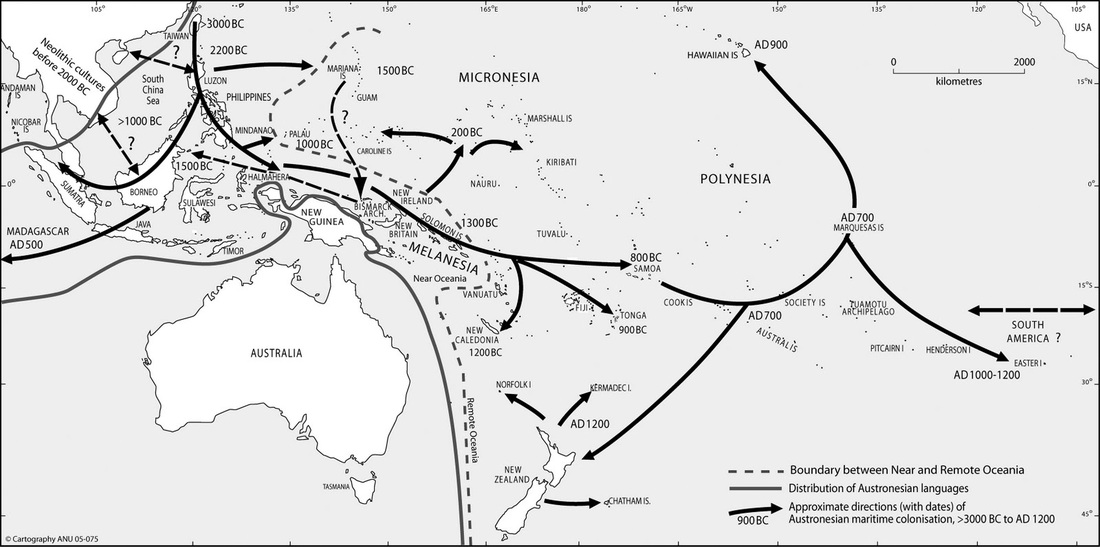
\includegraphics[width=\textwidth]{ANU_cartography.jpg}
\caption{Map of the expansion of the Austronesian language family, based on work by Peter Bellwood. Map made by ANU CartoGIS and Peter Bellwood.}
\label{austro_expansion_bellwood}
\end{figure}

Recent studies of ancient and modern DNA \citep{lipson_harvad_ancient_dna_vanuatu_2018, posth_jena_ancient_dna_vanuatu_2018} have shown that there is evidence of significant levels of genes that are associated with origins in non-Austronesian speaking communities from New Guinea and Solomons among Vanuatu people. The suggestion is that while the initial settlement of Remote Oceania was likely to be wholly Austronesian (i.e. genetically similar to East Asian populations), there have since been more people coming who have deeper ancestry from the New Guinea region. Interestingly, \citet{posth_jena_ancient_dna_vanuatu_2018} highlight that this had little effect on the languages of the region, communities in Vanuatu still speak languages that are clearly Austronesian in origin. This could be because the New Guinea people already spoke Austronesian languages at the point of migration or due to other reasons (cf. \citet[288, 321]{barlow2023papuan}; \citet[209-210]{bedford2018ancient}).

Likewise, further studies such as \citet{liu2022ancient} show similar genetic influence from New Guinea and Solomons northwards in Palau, Chuuk and Pohnpei island groups. It is becoming increasingly clear in the overall scientific literature on the ancient history of Oceania that there were a lot more connections and interactions than previously postulated --- including to island groups of Near Oceania. It is not the case that people travelled to one place, and then stayed put there with little influence from other people of Oceania. Oceania is an interconnected place today, and it was historically too.

It is possible that these interactions, which were more frequent in Vanuatu than in Polynesia, have implications for many domains of human life --- including political organisation and language diversity. Linguist and anthropologist \citet[104]{lynch1981melanesian} has stressed the relevance of contact with non-Austronesian communities from New Guinea, Bismarck, Bougainville and the Solomon Islands as a key factor in explaining why there are more languages in Vanuatu compared to the rest of Oceania \footnote{\citet{lynch1981melanesian} uses the terms ``Papuan'' and contrasts Melanesia and Polynesia. I have chosen to summarise him here in more precise terms in relation to how his work impacts the current study. He writes specifically about the influence of languages of New Britain, Bougainville, central Solomon Islands, Manus and the southeast of New Guinea mainland (Oro province, Milne Bay province and National Capital District) on Oceanic languages of those regions and in Temotu.}. Lynch does not offer a precise account but outlines several different potential scenarios whereby contact with non-Austronesian groups caused greater diversification among Oceanic languages.

Unfortunately, it is difficult to incorporate data on contact with non-Austronesian speakers explicitly in the models of this study. This is primarily due to lack of information on this variable in island groups such as Kanaky (New Caledonia), Ratak \& Ralik (Marshall Islands), Marquesas, Aotearoa and other island groups. However, this factor is very important and we will return to it in the discussions.

%could have impacted the differences in language diversification rates that we see in the region. However, unfortunately, there is not enough data for this to be included as a factor in the analysis of this study but it may be approximated by proxy-variables such as time depth of settlement


%\emph{\textcolor{red}{(Note to Andy, Simon, Mark and Nick: it is possible to include Papuan contact as a rather granular variable in the analysis. I have tried running a variable that just classifies each island group as "Melanesian" or "Not Melanesian" for example. That variable did not come out as significantly predicting the language diversity. It also felt a bit too crude. I talked to Beth about it and she recommended me to leave it out. However, if you would like I can keep it in and give caveats. I don't know yet of any DNA study that I can use for this. Both Posth et al and Lipson et al don't sample New Caledonia or Fiji at all, which makes it tricky to use here.)}}

%\footnote{Note that this is separate from theories of effects of culture and environment on the \emph{nature} of language, such as the work by \citet{wraygrace2007}, \citet{lupyandale2010} and \citet{raviv2019compositional}. Their work focusses on why different kinds of interactional patterns has consequences for the compositionality/complexity of a language. For this study, we are concentrating on linguistic \emph{diversity} as opposed to \emph{disparity}.}.

Finally, there has been a growing interest in environmental effects on language diversification\footnote{For a longer summary of recent studies of language diversification, see \citet{gavin2013toward} and \citet{greenhill2015demographic}.}. One of the oldest and most influential bodies of work in this vein is by Nettle. \citet{NETTLE1998} showed that there is a correlation between number of languages per country and ecological risk (as measured by mean growing season). Nettle suggests that high-risk environments encourage wider social networks and therefore reduce the number of languages in that area. \citet{hua2019ecological} expanded on this idea and explained that ``Smaller social groups are presumed to be more likely to be stable and self-sufficient in areas with a more abundant and reliable year-round food supply.'' \citet{hua2019ecological} constructed a more complex and fine-grained model of how environmental factors influence language diversity. They found that factors associated with risk (precipitation and temperature seasonality and season length) did indeed predict much of the distribution of languages in the world. Similarly, \citet{gavin2017process} showed that a simple model that takes into account rainfall and an upper bound of population size can to a large extent predict the distribution of indigenous languages in Australia. Given the success of these models, the amount and seasonality of rainfall and temperature variables are also included in our model predicting language diversity in Remote Oceania. 


%There are many more papers on demographic, cultural and environmental factors on language diversification, unfortunately there is not space enough here to relate them all. There are two overview papers that summarises many other studies on the topic very well --- \citet{gavin2013toward} and \citet{greenhill2015demographic}. I will refrain from copying their clear and instructive summaries and meta-analysis and instead direct the curious reader to seek those two papers out themselves should they want to explore the topic further.

In their study of global environmental predictors of language diversification, \citet{hua2019ecological} noted that there were certain areas that remained unexplained (New Guinea, Himalayas, West Africa and Mesoamerica). This may be an indication that the model needs to be adjusted to account for more variables or that the variables do not have the same effect globally. A recent study of language diversification in North America \citep{Pacheco_Coelho_2019} showed that the best predictors of language change may vary from place to place and that the factors are interlinked causally in a complex manner. Their study included environmental variables and data on the population. The authors note that political complexity might be an important variable too, but they were, unfortunately, unable to include it \citep[7]{Pacheco_Coelho_2019}.

This study focuses on a particular hypothesis concerning a particular region of the world. It is possible that these models perform less well globally and the results should primarily be compared against the specific theories of \citet{lynch1981melanesian} and \citet{pawley81, pawley2007} about Remote Oceania. As one of the few studies to include data on both environmental and socio-cultural variables, it is able to contribute a valuable perspective to the field of language diversity mechanics.

\FloatBarrier

%The cultural variables in this study are taken from D-PLACE \citep{d_place_all}, environmental data from ecoClimate \citep{ecoclimate} and archealogical dates from \citet{rieth_cochrane_2018}. The cultural variable of ``political complexity'' has been complemented with datasets from \citet{sheehan2018coevolution} and ethnographic sources. The archaeological dates were also further supplemented with data from \citet{levin_seikel_miles_2019, pol_outliers_stat_art, intoh2008ongoing, intoh2007reconnaissance} and \citet{Napolitano_et_al_yap}. 


%We will also be using two environmental variables taken from D-PLACE: Net Primary Production (NPP) and NPP predictability. The Net Primary Production is the grams of carbon uptake per square meter of land per month.
\FloatBarrier
\section{Materials and Method}
\label{pol_complex_method}
The approach of this paper is to gather relevant data on island groups and their societies and then fit statistical modeld which aims to predict the number of languages given all the variables. From the composition of variables in the resulting model we can infer which have the greatest predicting power when they are co-estimated.

The unit of analysis is ``island group''. We cannot use modern political boundaries (``French Polynesia'', ``Cook Islands'' etc) because they are often historically and culturally inappropriate. As we want to capture something about the communities at large we are not satisfied with using individual islands. For these reasons, we use two different ways of grouping islands: overnight sailing distances and shared language (see appendix \ref{appendix_sec:island_geo} for details).

%Predicting_lgs_DAG_full

A simple test of Spearman's Rank Order correlation reveals that the number of languages and political complexity per island group are indeed moderately correlated (rho  = -0.4, \emph{p} value < 0.001 for islands grouped for shared language). However, this is not sufficient. We want to investigate whether this correlation still holds once we explicitly incorporate other variables that we expect might explain language diversity as well, such as time-depth and environmental factors. In addition, we also include controls for phylogenetic and spatial non-independence in order to account for unobserved confounds that may be transferred through contact or inherited and affect the number of languages (cf. \citet{gavin2013toward}).

Variables were included in the model if they meet all three of the following criteria: a) have been suggested as relevant in previous literature, b) there is enough data on most of the island groups in a published source and c) if they relate to the response variable (language richness) in a non-mediated manner (cf. \citet{pearl1995causal} and \citet{cinelli_et_al_2022}). Figure \ref{appendix_Predicting_lgs_DAG_full} in the appendices shows the full set of variables that were considered and figure \ref{appendix_Predicting_lgs_DAG_slimmed}, also in the appendices, the ones that ended up being implemented. This filtering resulted in the following variables:

\singlespacing

\begin{itemize}
\item \textbf{response variable}:
\begin{itemize}
\item \textbf{number of languages} - language classification based on \citet{glottolog40} and other sources (see Appendix \ref{appendix_sec:language_class}).
\end{itemize}
\item \textbf{predicting variables:}
\begin{itemize}

\item \textbf{EA033} - number of vertical levels of jurisdictional hierarchy per society\footnote{Note that there are other kinds of political complexity besides vertical, for example, horizontal complex exchange networks and this variable only tracks hierarchy. See Appendix \ref{appendix_def_pol_complex} for more details.}, based on the Ethnographic Atlas \citep{gray1998ethnographic, d_place_all}, \citet{sheehan2018coevolution} and own modifications. Also known as ``political complexity'' (see appendix \ref{appendix_def_pol_complex} for details on definition and coding).

\item \textbf{Settlement time depth} - archaeological dates, grouped into waves \citep{intoh2007reconnaissance, intoh2008ongoing, rieth_cochrane_2018, levin_seikel_miles_2019, pol_outliers_stat_art, Napolitano_et_al_yap}. (See appendix \ref{appendix_def_dates} for details.)

\item \textbf{Shoreline} - length of shoreline of landmasses from the Global Self-consistent, Hierarchical, High-resolution Geography Database (GSHHG) \citep{wessel1996global} (see appendix \ref{appendix_environ} for details.)

\item \textbf{Environmental Principal Components} - based on variables related to how suitable the islands are for human settlement


\begin{itemize}
    \item \textbf{temperature and rainfall} - historical environmental data from \citet{ecoclimate}: mean temperature, temperature seasonality, mean rainfall and rainfall seasonality (see appendix \ref{appendix_environ} for details.)
    \item \textbf{Net Primary Productivity} - derived from data from NASA satellites Terra and Aqua \citep{running2021modis_aqua, running2021modis_terra} (see appendix \ref{appendix_environ} for details.)
    \item \textbf{Absolute latitude} - based on the Global Self-consistent, Hierarchical, High-resolution Geography Database (GSHHG) 
\end{itemize}


 \item \textbf{Phylogenetic non-independence} - based on the median of patristic distances between languages of different island groups. Phylogeny based on Glottolog v5.0 \citep{Glottolog5}, with branches modified with Grafen's transform.
 
\item \textbf{Spatial non-independence} - based on the minimal haversine distance between landmasses of island groups

\end{itemize}

\end{itemize}

\doublespacing

The variables Net Primary Production (NPP; the amount of biomass or carbon produced), temperature \& rainfall (mean and seasonality) and absolute latitude are all associated with the suitability of a place for life and they correlate with each other, at least to some degree (cf. Figs \ref{appendix_SPLOM_medium_all_variables} and \ref{appendix_SPLOM_SBZR_all_variables}). In this study, they are all tracking a similar concept: the suitability for human populations to thrive in smaller groups. Because of this, we are running a Principal Components Analysis on all variables related to this concept (NPP, temperature, rainfall and absolute latitude), this allows us to extract a variable that explains most of the information. The aggregation is carried out twice, once for values of islands grouped by overnight-sailing distances and one for groups based on shared language. We ran a Non-Graphical Cattel's Scree Test \citep{cattell1966scree, R-nFactors} to determine the number of optimal components (overnight sailing distance island groups = 2 PCs, shared language island groups = 3 PCs). For more details, see Appendix \ref{appendix_environ}.

In order to create a formula for the statistical model, we consider the suggested causal relationships based on previous research (see section \ref{sec:previous_research}). Besides the effect of the environmental variables on language richness, we also hypothesise that there can be a joint effect with the size of the island. Similarly, the time-depth and size of islands may also interact. 

The relationship between variables is represented in DAG in Fig. \ref{appendix_Predicting_lgs_DAG_slimmed} in the appendix. For the full DAG, including excluded variables and variables with missing data, see appendix \ref{appendix_DAG_def}. Interactions are denoted with a deterministic node labelled with $\ast$. 

This results in the model formula below. The formula is formatted in the style and conventions of statistical programming in R. The response variable is to the left of the tilde ($\textasciitilde{}$) and the different predictors are combined with + for additive factors and with $\ast$ for interactions. Environmental PC3 is only included for the models predicting the number of languages of islands defined by shared language (based on the outcome of the Non-Graphical Cattel's Scree Test). The models are also run with and without control for phylogenetic and/or spatial non-independence. Predictors that are only in some of the models are marked with parentheses.

\begin{quotation}
\texttt{Number of languages \textasciitilde{} EA033 +} \\
\indent \indent\texttt{Settlement order *  Shoreline +} \\
\indent \indent \texttt{Environmental PC1  *  Shoreline +} \\
\indent \indent\texttt{Environmental PC2  *  Shoreline +} \\
\indent \indent (\texttt{Environmental PC3 *  Shoreline +}) \\
\indent \indent (\texttt{Phylogenetic relations +}) \\
\indent \indent (\texttt{Spatial relations }) \\
\end{quotation}

Settlement order was reversed from Fig. \ref{appendix_dates_map} such that high numbers represent further back in time, making the interpretation of effects more intuitive. Shoreline was log-10-transformed to reduce the effect of extreme outliers such as the South Island of Aotearoa (cf. \citet{rolett2004environmental} and \citet{atkinson2016cultural}). For EA033 (political complexity), the mode of each island group was used\footnote{In instances of ties, the value for the island group was randomly selected.}. All predicting variables were then normalized in the conventional manner by subtracting the mean and dividing by the standard deviation (centering and scaling). EA033 and settlement waves were both modelled as monotonic effects (i.e. it is not assumed that the difference between level 1 and 2 is the same length as the difference between 2 and 3, but they are still on an ordinal scale).

To test the impact of several variables predicting the same response variable we use a Bayesian Regression Model \citep{gelman2006data, burkner2017brms}. The distribution of languages per island group is over-dispersed; there are many island groups with one language and only a few with higher numbers (see Figs. \ref{appendix_polygon_plot_SBZR} and \ref{appendix_polygon_plot_medium} in Appendix \ref{appendix_sec:island_geo}). For the overnight-sailing island groups, the group that contains Vanuatu and Temotu has 130 languages, whereas most island groups in Polynesia have 1 or 2 languages each. This skewed distribution necessitates a Poisson distribution for the response variable in the model, which is able to adjust the relationship between the mean and the variance appropriately (c.f. \citet{winter2021poisson})\footnote{This issue was also faced by \citet{gavin2012island} in their study of environmental factors in language diversification in the Pacific. They chose another approach, a reciprocal transformation, based on model fitness compared to two other kinds of transformations of the response variable. We chose to manipulate the response variable as little as possible to keep the model and its interpretation as intuitive as possible also for readers with less advanced knowledge of statistical modelling.}. For further details on the model set-up, see appendix \ref{appendix_model_settings}.

Due to missing data on some island groups, we are testing our models over 65 out of 104 shared language groups and 56 out of 67 overnight distance groups. This sample still contains some of our more extreme sites, like Santo, Kanaky (New Caledonia mainland) and Malakula. Variables that did not cover Vanuatu and New Caledonia with enough specific data points are not included in this study, for example historic population data, non-Austronesian gene flow or jurisdictional hierarchy within local communities (as opposed to beyond local community which is what EA033 covers). 

To test the robustness of the conclusions over all observations, we drop one observation out at a time and calculate the predictor effects and predictions of the number of languages. This allows us to assess which island groups represent the largest challenge to the model and may indicate areas where further in-depth study is necessary. 

For each kind of grouping of islands (shared language and overnight sailing) four models were run (no control for spatial or phylogenetic non-Independence, spatial control, phylogenetic control and control for both spatial and phylogenetic non-independence). This results in 8 models in total. For each island grouping, the four models are compared to each other using Leave-One-Out cross-validation (LOO), Watanabe–Akaike Information Criterion (WAIC), Bayesian $R^2$ and mean absolute difference between predicted and observed number of languages (similar to accuracy). LOO and WAIC were computed following  \citet{vehtari2017practical}, as implemented in the R-package loo \citep{R-loo}, Bayesian $R^2$ following \citet{gelman2019r} as implemented in the R-package rstanarm \citep{R-rstanarm}

The results were calculated in R 4.3.3 \citep{R} using the function \texttt{brms::brm()} \citep{burkner2017brms} and the tidyverse suite of R-packages \citep{tidyverse13}. For a full list of packages used and their versions, see appendix \ref{appendix_r_packages}.

\FloatBarrier
\section{Results}
The results show that EA033 has a significant effect in some of the models, but not all. This lends support to the proposal by \citet{pawley81, pawley2007}. However, there are details of the result that suggest that the effect may be due to non-Austronesian contact rather than political complexity \emph{per se}.

The model comparisons showed that the models without control for spatial and/or phylogenetic non-independence fit the data less well. The model fit scores were overall similar for the other models (see appendix 
\ref{appendix_model_fit_scores}). Table \ref{brms_results_summary} shows whether or not EA033 and/or EA033 in interaction with shoreline (EA033:Shoreline) had a significant effect in each model (i.e. 95\% confidence interval of the posterior effect distribution does not straddle zero) and the WAIC scores of each model. The model fit scores reported very similar ranking of the models, in the table \ref{brms_results_summary} only WAIC is included but the others can be found in Appendix \ref{appendix_model_fit_scores}.

\begin{table}[ht]
\centering
\begin{tabular}{p{2.2cm}p{2.6cm}|p{2.2cm}p{2.2cm}p{2.2cm}p{2cm}}
  \toprule
&&  \multicolumn{4}{c}{\textbf{Control for spatial and/or phylogenetic non-independence}}\linebreak\\
 & \textbf{	Variable	} & \textbf{	none	} & \textbf{	phylo	} & \textbf{	spatial	} & \textbf{	spatialphylo	} 	\\
\midrule
\multirow{2}{*}{Shared language}
 	&	Significant effect	&	\cellcolor{spec_color_lightgreen!50} EA033  \& EA033:Shoreline	&	\cellcolor{spec_color_lightgreen!50} EA033:Shoreline	&	\cellcolor{spec_color_lightgreen!50} EA033 &	Neither		\\
		&	WAIC	&	231.952	&	208.562	&	209.082	&	 207.749		\\
  \midrule
\multirow{2}{*}{Overnight sailing}	&	Significant effect\linebreak	&	\cellcolor{spec_color_lightgreen!50} EA033:Shoreline	&	Neither	&	\cellcolor{spec_color_lightgreen!50} EA033:Shoreline &	Neither		\\
	&	WAIC	&	191.558	&	 172.586 	&	178.292	&	173.43		\\


   \bottomrule
\end{tabular}
\caption{Summary of results in regards to variables of interest (EA033 alone and in interaction with Shoreline). Significant effect means that the 95\% confidence interval of the effect does not straddle zero (marked in green). The model fit can be compared using the Watanabe–Akaike Information Criterion (WAIC). Lower WAIC-values indicate a better model fit.} 
\label{brms_results_summary}
\end{table}



We will first go through the outcomes for the shared language island groups (i.e. groups of islands that share at least one language), and secondly the overnight distance groups. In common for both is that political complexity is a relevant predicting factor in some of the models, with a negative effect (the more political vertical levels, the lower the number of languages). This lends support to the proposal by \citet{pawley81} and \citet{pawley2007}. However, there are details of the result that suggest that the effect may be due to non-Austronesian contact rather than political complexity \emph{per se}.



% BARG

Fig.~\ref{medium_model_predict} shows the actual observed language counts (purple triangles) and predictions of this model (green boxplots\footnote{The green box-plots represent the posterior predictions from the model (10,000 draws). The plot follows conventional design for box-plot, with the middle of the box representing the median, the two ends of the box (a.k.a ``hinges'') the first and third quartiles (the 25th and 75th percentiles). The whiskers extends from the end of the box 1.5 $\ast$  of the distance between first and third quartiles. Data beyond the end of the whiskers, so called "outlying" points, are not visualised in this plot as they were found to give a biased impression of the range. The R-function  ggplot2::geom\_boxplot() was used for these visualisation, scripts are included in additional material.}). The model does predict that Santo, Kanaky and Malakula have the highest language counts in the dataset. Our observed language counts for Santo, Kanky and Malakula are 24, 29 and 33 respectively. The model is very close for Santo and Kanaky for its average prediction value but underestimates Malakula by 17 languages. The absolute average difference between the mean predicted values and the observed is 1.3.

%The results show that the model run with the shared-language island groups have an absolute average of difference between the predicting number of languages and observed of 2,8 the overnight-sailing distances island groups of 4.3 Fig.~\ref{medium_model_predict} and Fig.~\ref{SBZR_model_predict} illustrate the specific predictions the models make compared to the observed language counts. 

\begin{figure}[ht]
\centering
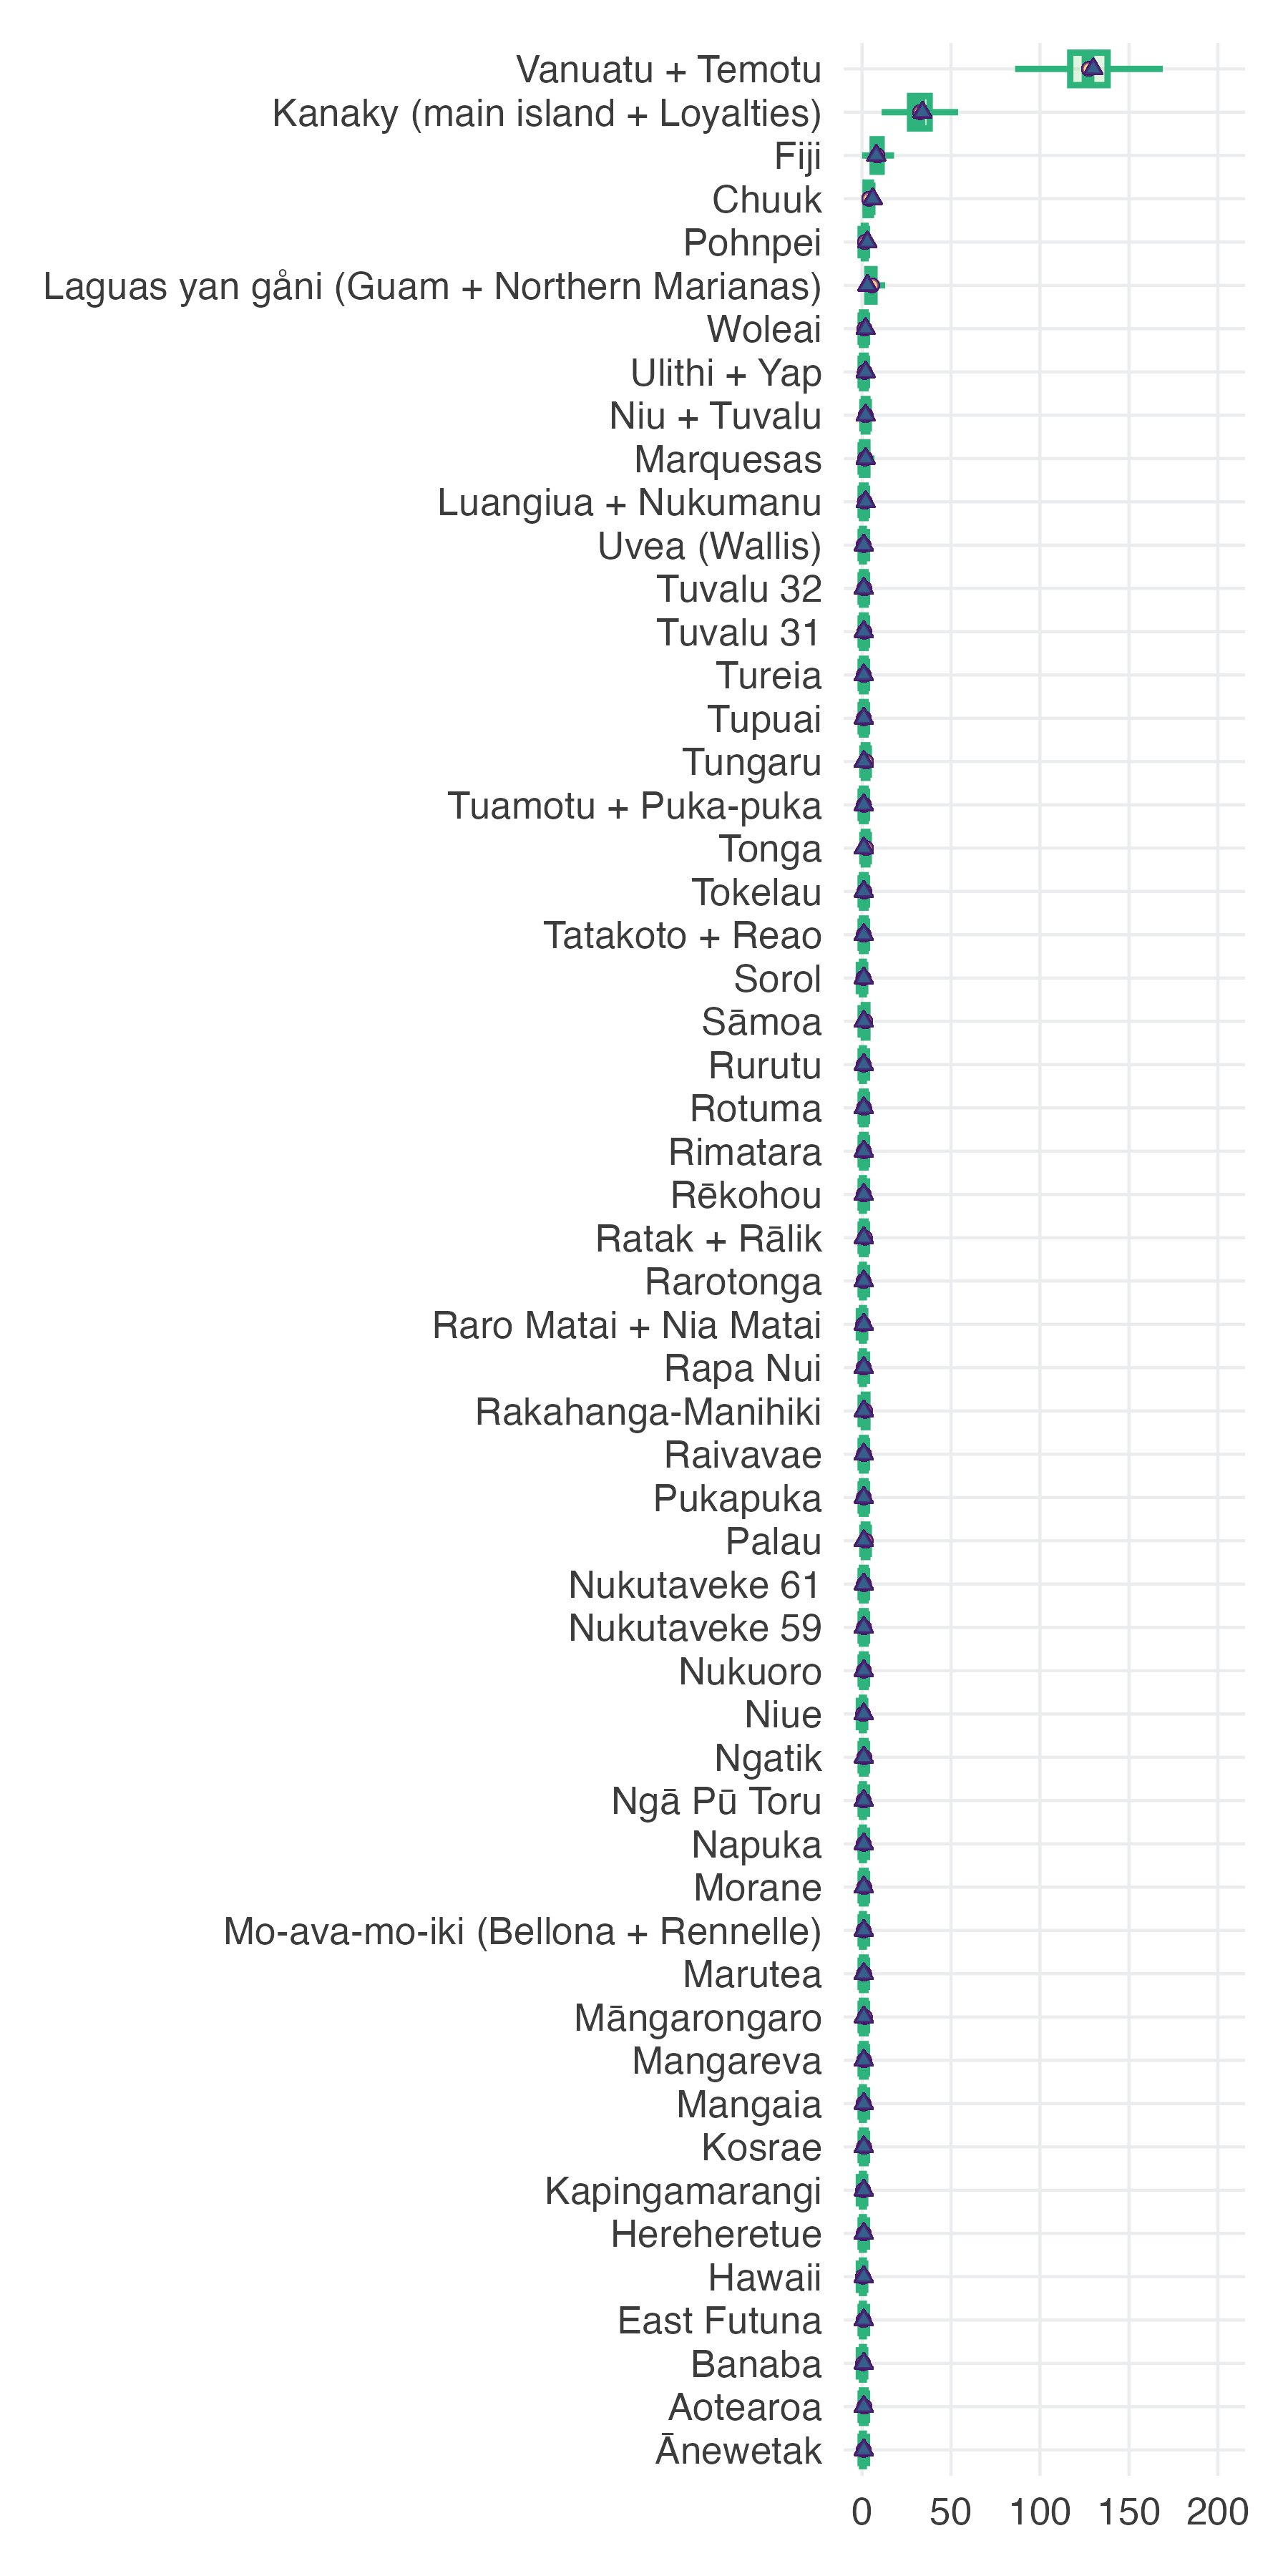
\includegraphics[width=0.6\textwidth]{latex/brms_predict_SBZR_control_spatialphylo.png}
\caption{Posterior predictions from the model with island grouped for shared language (10,000 draws). Number of languages is on the x-axis, observations on the Y. The dark blue triangles represent the observed number of languages, the green boxplot the predictions of the model. The middle of the box represents the median. The mean is represented with a yellow circle.}
\label{medium_model_predict}
\end{figure}

For the shared language island groups, the variables that have a 95\% confidence interval which are not different from zero are: political complexity (EA033), environmental PC1, Shoreline, time depth and shoreline in interaction with time depth. Fig \ref{brms_SBZR_group_full_effect_ridge_panels} in Appendix \ref{appendix_supp_figs} shows the full distributions.

\begin{figure}[ht]
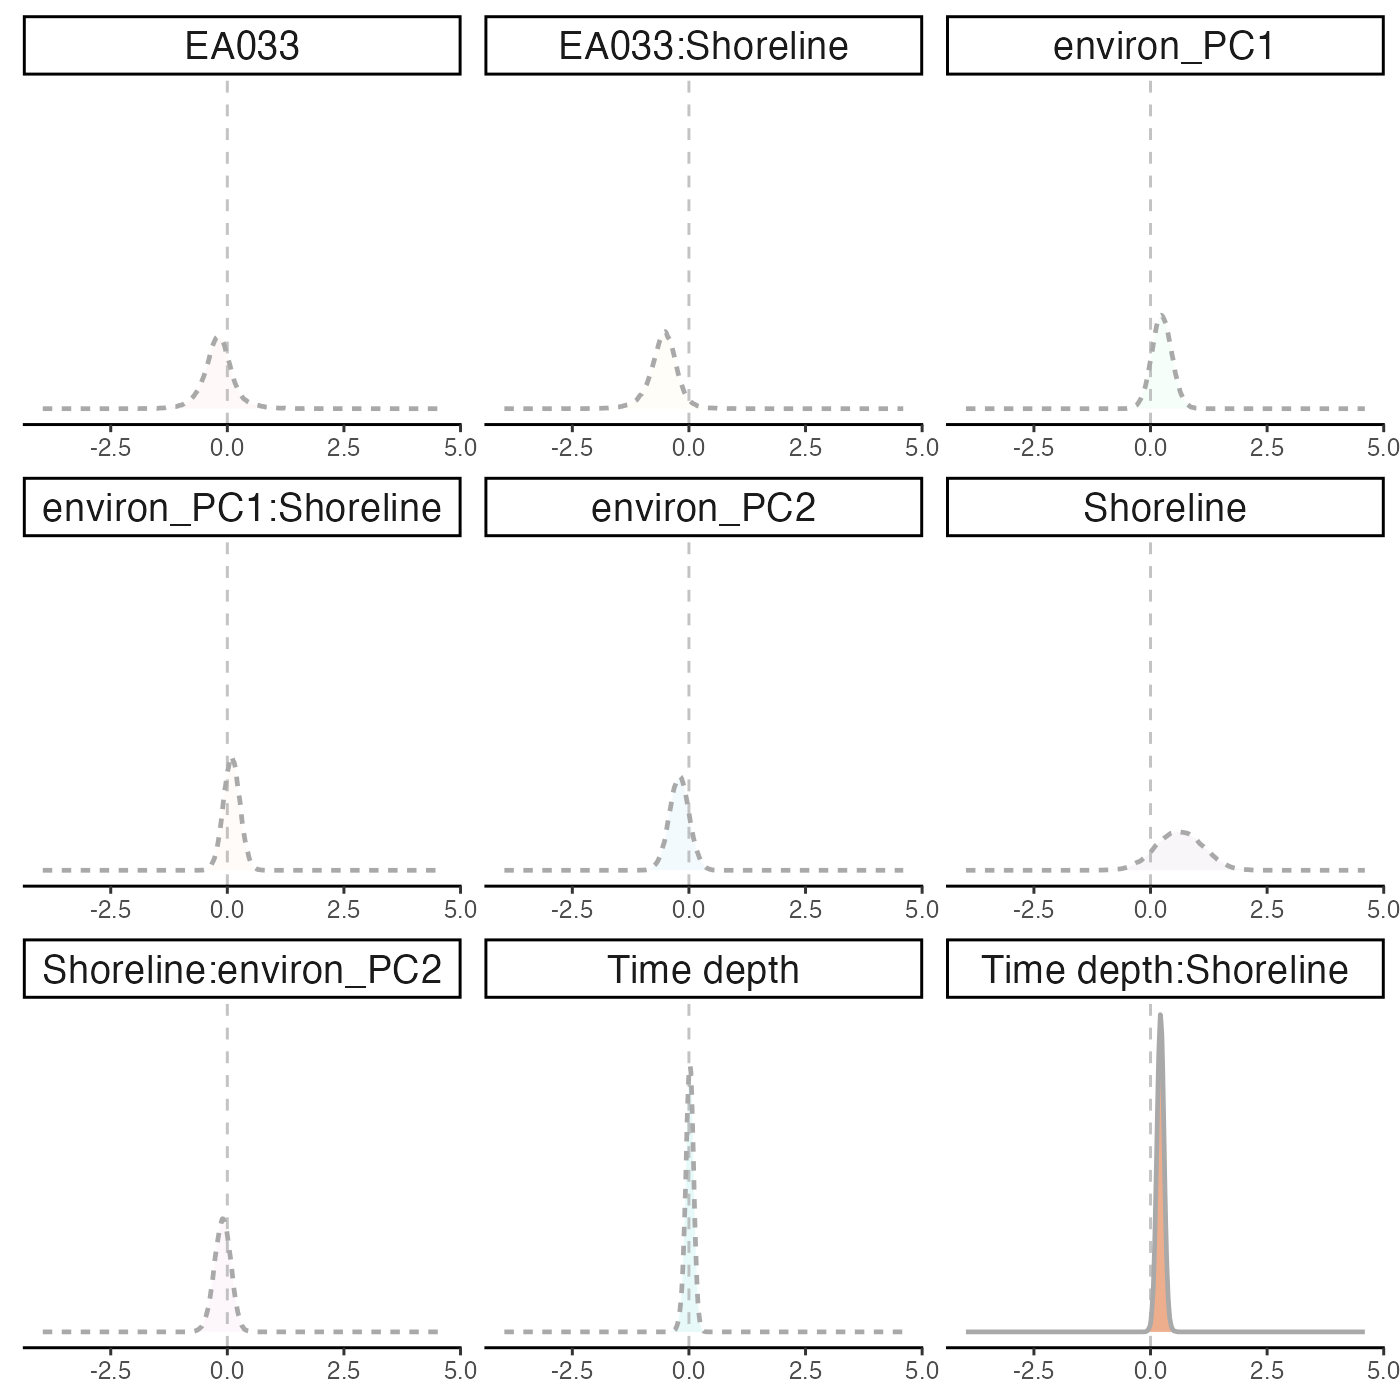
\includegraphics[width=0.6\textwidth]{latex/brms_SBZR_control_spatialphylo_group_full_effect_ridge_panels_plot.png}
\caption{Coefficient distribution of BRMS model, using overnight sailing distances island groups with all observations - including control for phylogenetic non-independence. Distributions, where the 95\% confidence interval straddles zero, are marked as more transparent and with dashed outlines.}
\label{brms_SBZR_group_full_effect_ridge_panels_phylo}
\end{figure}


\begin{figure}[ht]
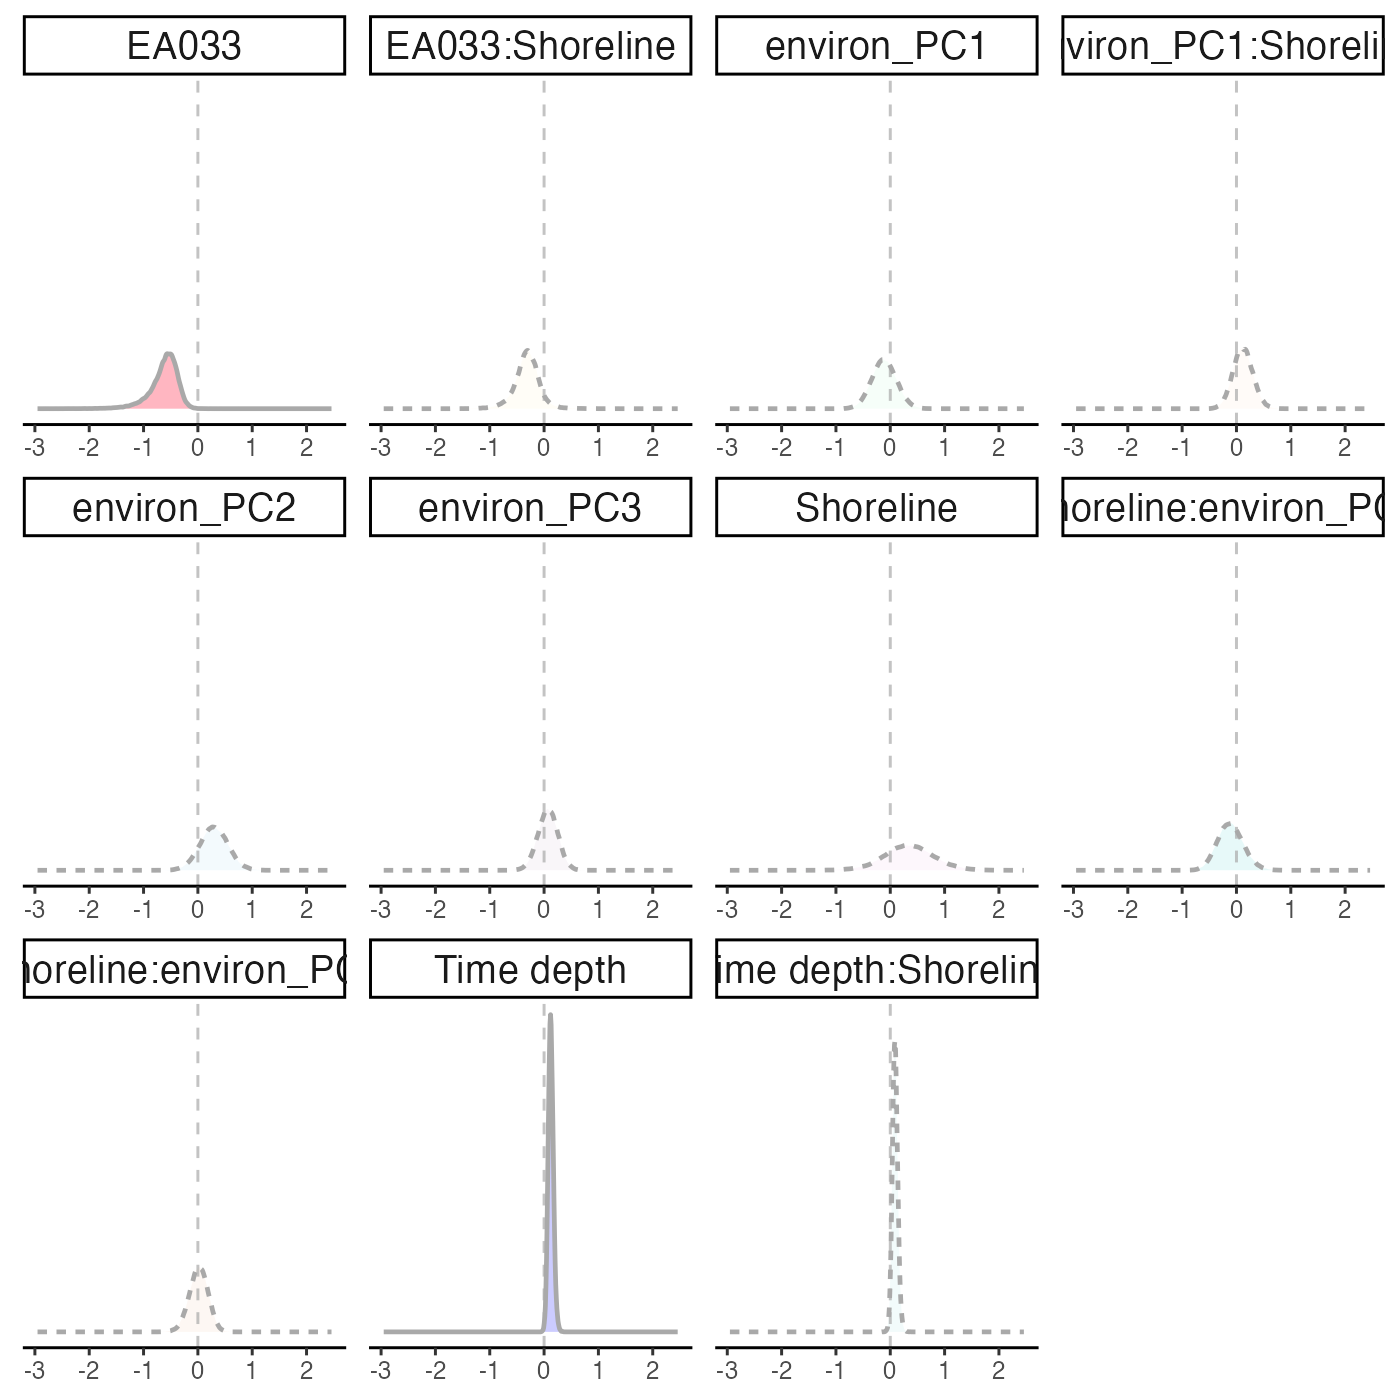
\includegraphics[width=0.6\textwidth]{brms_medium_control_spatial_group_full_effect_ridge_panels_plot.png}
\caption{Coefficient distribution of BRMS model, using shared-language-distances island groups with all observations - including control for spatial non-independence. Distributions, where the 95\% confidence interval straddles zero, are marked as more transparent and with dashed outlines.}
\label{brms_SBZR_group_full_effect_ridge_panels}
\end{figure}







% #Frederic says: could also compute pareto-k https://mc-stan.org/loo/reference/pareto-k-diagnostic.html

Most of the island groups can be removed with little effect on the overall accuracy of predictions (see Fig.  in \ref{appendix_supp_figs}), however, when Malakula (central Vanuatu), is left out, the difference average difference between predicted and observed becomes lower (1.3 $\rightarrow$ 0.9). Malakula is the island group with the highest number of languages (see Fig \ref{appendix_polygon_plot_medium} in appendix \ref{appendix_sec:island_geo}). Political complexity remains an important predictor regardless of which island group is dropped.

%and shoreline in interaction with time depth are the variables that have a significant impact, i.e. do not cross zero (see coefficent distributions in Figs.  and \ref{brms_medium_group_full_effect_ridge_panels} in appendix \ref{appendix_supp_figs}).

For the overnight sailing distances, several island groups are much larger than the previous grouping. The islands of Vanuatu  (including Anuta and Tikopia) and Temotu are all within the same group (see Fig \ref{appendix_polygon_plot_SBZR} in appendix \ref{appendix_sec:island_geo}; this is similar to the groups considered in \citet{pawley2007}). This also leads to a larger discrepancy between the number of languages, with Vanuatu and Temotu having 130 and S\={a}moa still only one. The average absolute difference between the predicted and observed number of languages is somewhat greater than for the previous grouping --- 1.6. Fig \ref{SBZR_model_predict} shows the prediction vs observed per island group.

\begin{figure}[ht]
\centering
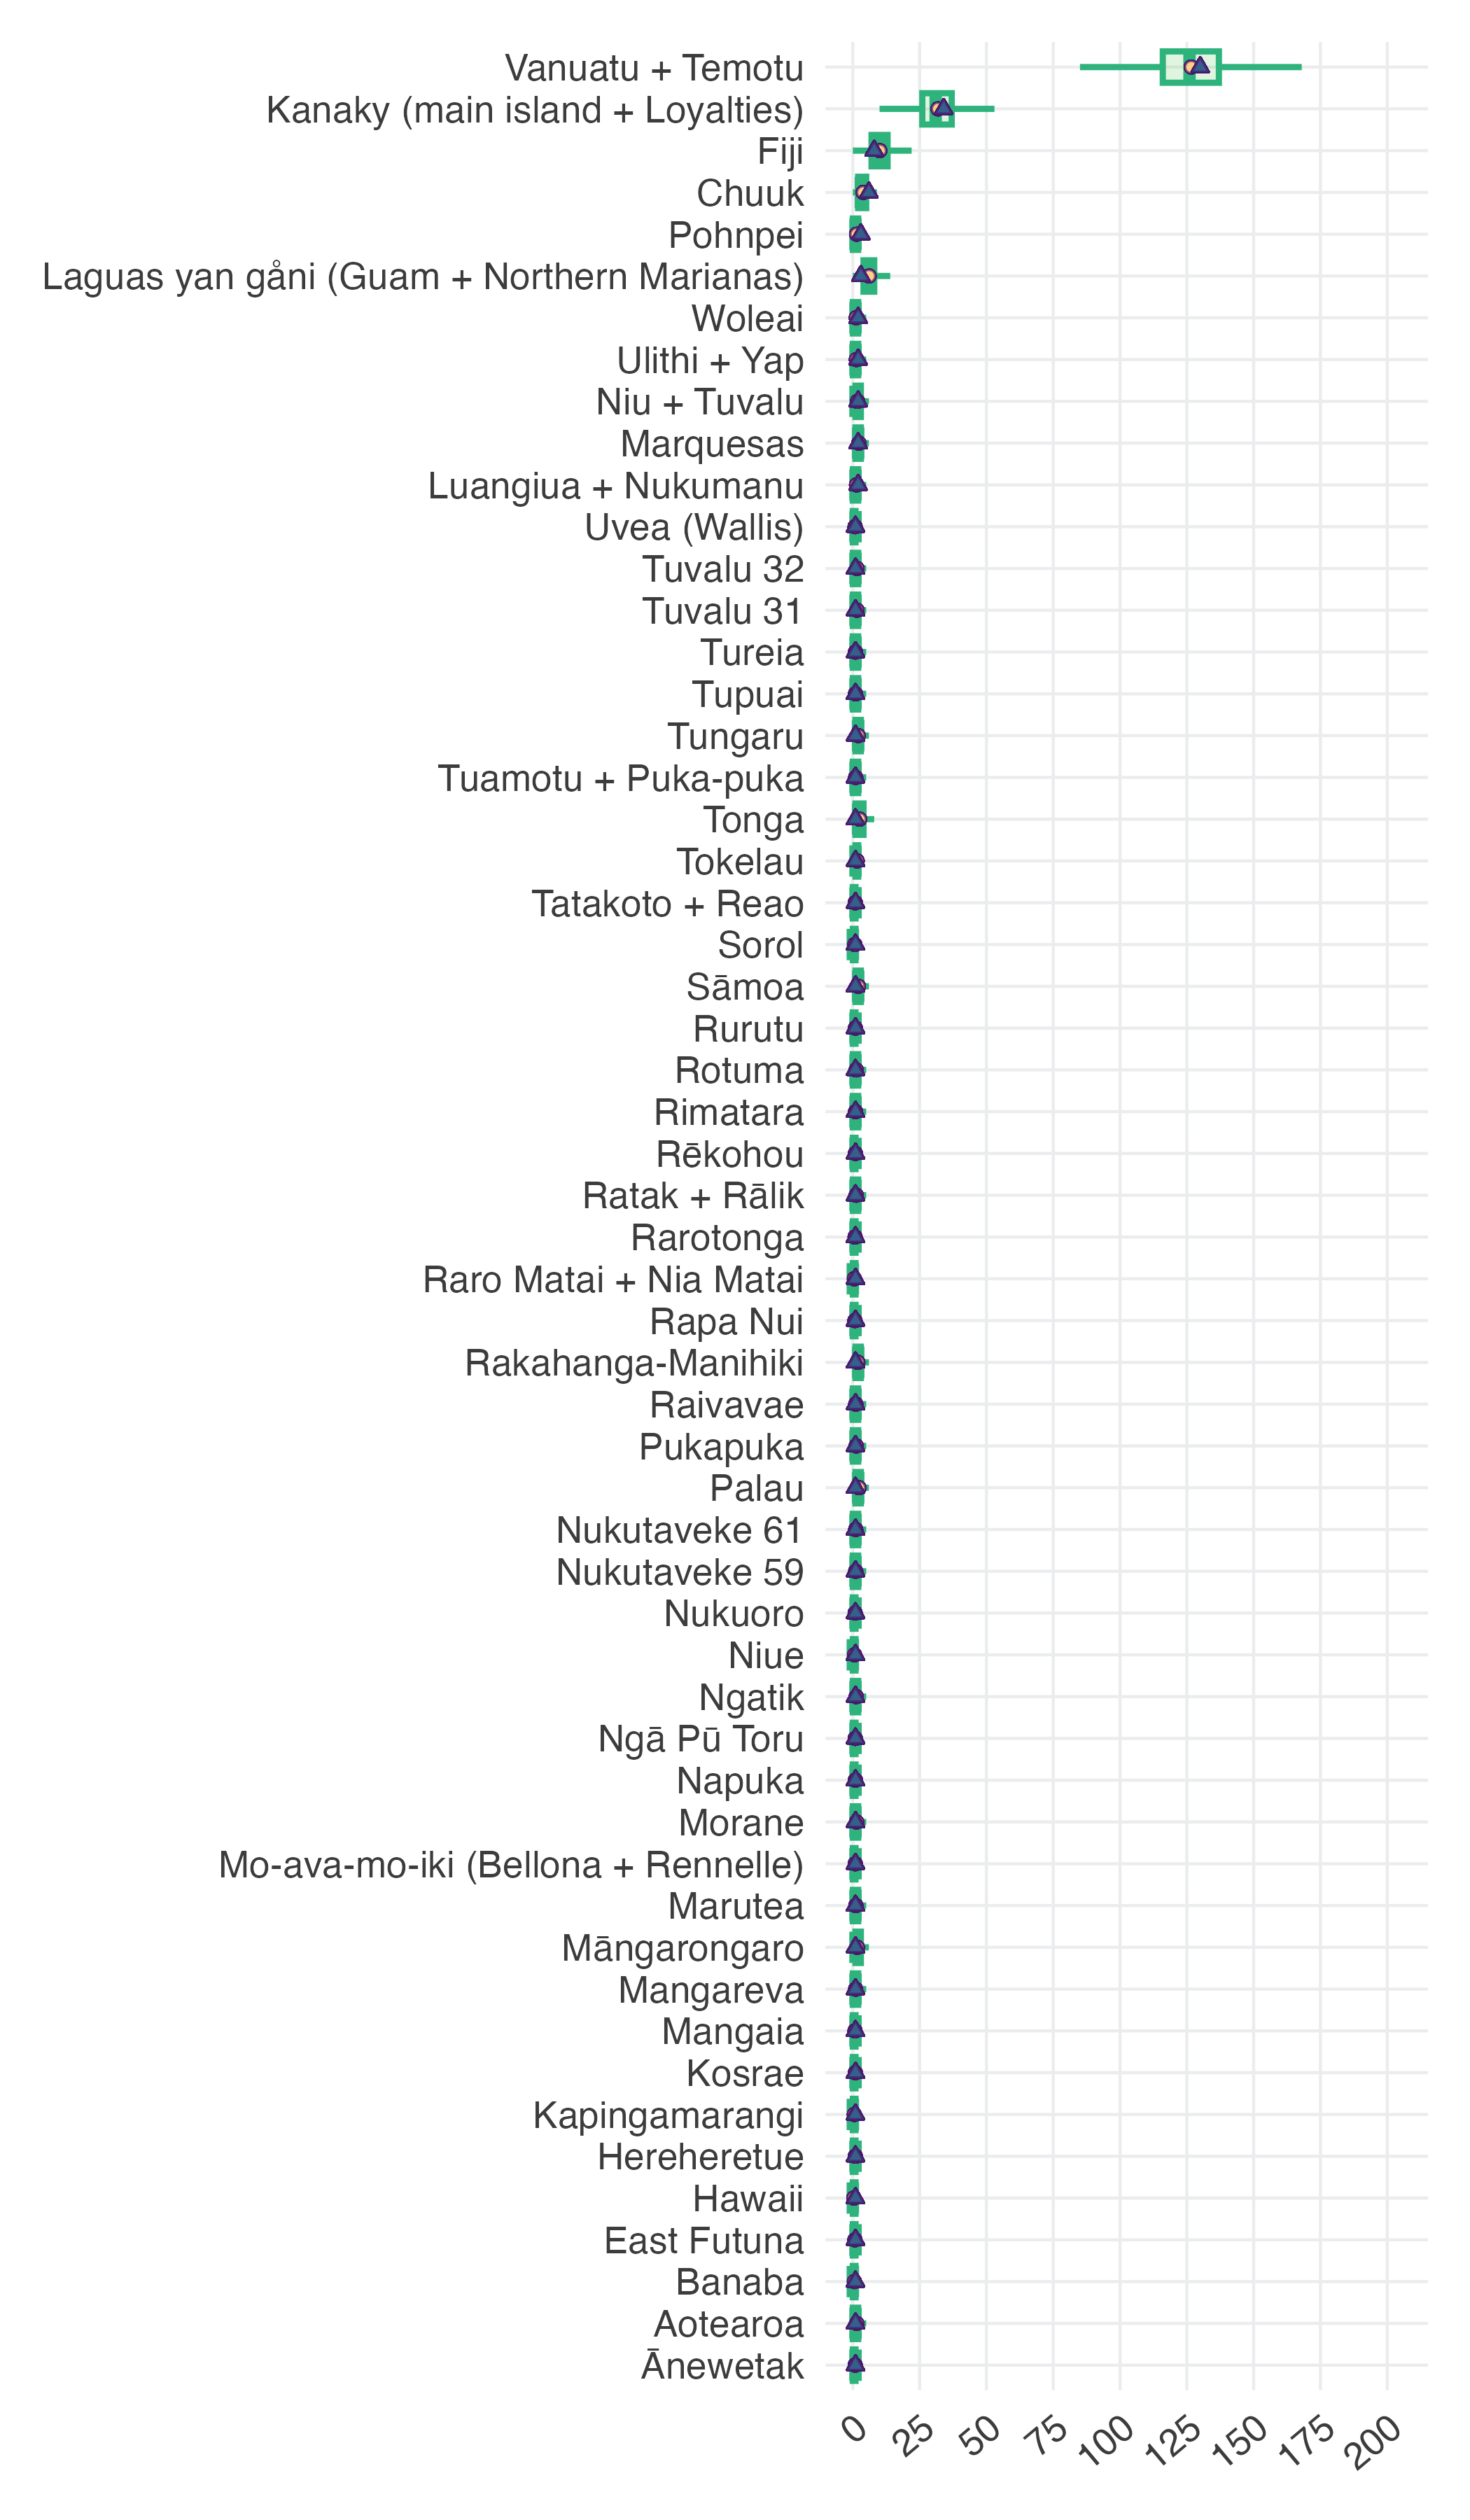
\includegraphics[width=0.6\textwidth]{latex/brms_predict_SBZR_control_spatial.png}
\caption{Posterior prediction from the model with island grouped for overnight sailing distances (draws = 10,000). The dark blue triangles represent the observed number of languages, the green boxplot the predictions of the model. The middle of the box represents the median. The mean is represented with a yellow circle.}
\label{SBZR_model_predict}
\end{figure}

%Shoreline:Settlement_date_grouping_finer§straddle_zero_95
%environ_PC1:Shoreline§straddle_zero_95

The most important variables in this model (i.e. 95\% confidence interval of coefficient distribution does not overlap 0) were: political complexity, environmental PC2, shoreline, time depth and time-depth in interaction with shoreline  (see Fig ). However, if we drop out Vanuatu + Temotu this no longer holds. When Vanuatu + Temotu are left out, the coefficient distribution of political complexity overlaps zero. Instead,  Shoreline in interaction with time depth and environmental PC1 in interaction with Shoreline are relevant predictors. When Vanuatu + Temotu are dropped out, the overall difference between predicted and observed values goes down the most (from 1.6 to 0.7, see Fig. \ref{appendix_brms_SBZR_dropped_out_plot_diff}). When Vanuatu + Temotu are excluded, the model is more accurate. If we ask this model that has been trained \emph{without} the Vanuatu + Temotu data to predict how many languages there are there, it grossly underestimates and proposes 7 languages (observed = 130). If we drop out any other island group (including Kanaky), political complexity remains an important predictor.

For tables of the predictor Estimates, Rhat and ESS of both models, please see appendix \ref{appendix_BRMS_model_tables}.

%Most of the island groups in this dataset have only one language, and this seems to have caused some issues (despite the Negative Binomial distribution). The model does best at predicting languages in Polynesia (which is dominated by island groups with only one language). Islands groups in Polynesia can have a very long coastline (like the Paumotu archipelago of French Polynesia) or very short one (like Niue). There is not as much difference in shorelines between islands of Vanuatu. The model seems to have struggled with using shoreline to predict languages globally, even leading to the result that Shoreline as a standalone term comes out in the model as negatively predicting the number of languages (though not with a \emph{p} value that passes traditional thresholds of significance). 

%Among the island groups the model predicted \textit{least} successfully is Paama, a very small island of Vanuatu with one language. The model predicted 5.2 languages, the observer value is one. 

%Paama is coded 1 for political complexity \citep{bonnemaison1996graded} and as part of the third wave of settlement \citep{rieth_cochrane_2018}. Most island groups that are coded as low for political complexity and low for settlement are found in Vanuatu and can be somewhat differentiated by Shoreline with Malakula and Santo having longer shorelines and more languages. However, in the full sample there are island groups with much longer shorelines and only one language (Aotearoa and Paumotu). The estimates of the model show that while the interaction of Shoreline and Settlement order has a significant positive influence as an interaction, the effect is not large.



%brms_SBZR_dropped_out_plot_diff


\FloatBarrier
\section{Discussion}
\label{pol_study_discisson}
The results indicate that political complexity could be relevant for understanding the dynamics of language diversification in Remote Oceania, but further studies are needed --- especially regarding Vanuatu. 

When the island group Vanuatu + Temotu was dropped, the model for overnight sailing island groups no longer drew on political complexity as a relevant predictor of language richness. This may indicate that it primarily made use of the variable to tell apart Vanuatu + Temotu from all other island groups. Vanuatu + Temotu is by far the island group with the most languages, 130, and it is dominated by societies that are classed as level 1 on the scale of vertical political complexity used by the Ethnographic Atlas \citep{gray1998ethnographic} and other studies \citep{watts_2018}, see Fig. \ref{appendix_pol_complex_map} in appendix \ref{appendix_pol_complex}).

Furthermore, if we tease apart the argument concerning political complexity (for example in the full DAG in Fig. \ref{appendix_Predicting_lgs_DAG_full} in appendix \ref{appendix_DAG_def} or Fig. \ref{Predicting_lgs_DAG_andy} in section \ref{sec:previous_research}), we find that conceptually the link between the number of languages and political complexity is not direct. It could be mediated through other factors such as network modularity, the propensity to maintain long-distance contact etc. 

\citet{watts_2018} found that politically complex societies in Oceania became Christian at a faster speed. This may indicate that changes propagate through a population quicker if the society is not egalitarian. If Christianity spreads faster in societies with higher complexity, it is possible to reason that other changes also might spread faster. If changes propagate quickly throughout a population, that leaves less possibility for diversification through natural drift or groups in the periphery staying more archaic compared to the centre. This interpretation relies on the understanding that the variable for political complexity (EA033) reveals something not only about jurisdictional power relationships in a given society, but also captures something about the social network of \emph{all} of its members (not just the leaders). Under this theory, people living in societies with higher political complexity would be able to travel further and have wider-ranging social networks, which in turn would lead to greater internal cultural homogeneity.

Maintaining long-distance contact can indeed be a function of shared cultural identity. \citet[218-291]{skirgaard2020multilevel} notes that there are not only fewer languages in the island groups of Polynesia, but they are also more similar to each other lexically than languages in Vanuatu are. This relationship does not hold for grammatical features however, languages in Polynesia are about as different from each other grammatically as languages of Vanuatu and other island groups in Remote Oceania are (as measured by Grambank features, \citep{grambank_release}). It has been suggested, by \citet{silverstein1981limits}, \citet{francois2011} and others (cf. \citet{mansfield2023dialect}), that communities pay special attention to words and sound differences as emblematic of shared ties --- but grammar tends to fly under the radar in this respect. This difference between Vanuatu and Polynesia in terms of lexical dissimilarity and language richness, but the similarity in terms of grammatical diversification may indicate that the cause does indeed lie in attitudes and social network organisation  - similar to the findings of this study.

\citet{curriemace2009} argue that the reason behind their results (higher political complexity = larger language areas) is that societies with higher political complexity are more likely to be able to replace existing groups in an area, or otherwise incorporate (and possibly assimilate) them. It may also be the case that diversity in Polynesia was reduced by later expansionist efforts by societies with higher political complexity. For example, the island of Niuafo'ou which lies between Tonga, 'Uvea and S\={a}moa is home to a language that is most closely related to 'Uvean. This language has however become \emph{more} similar to Tongan during the period of Tongan domination in the area 1000-1300's (see \citet{aswani1998tongan} and \citep[2-9]{tuskamoto_niuafoou}). It may be that politically complex societies do not only \emph{maintain} homogeneity by continuing to be in contact after first settlement, but can also reduce diversity which emerges after settlement through incorporation and cultural dominance later.

Whatever the political complexity variable is tracking, it is clear that it is one of the variables that most clearly picks out Vanuatu and that Vanuatu is the place with the most languages. Where did this difference in societal organisation come from? As previous studies have indicated (e.g. \citet{lynch1981melanesian}), the answer may lie in contact with people of non-East Asian origin further west. It is possible that contact with communities from New Guinea and Solomons (in Bismarck before migration to Vanuatu or in Vanuatu after initial settlement) brought with it societal changes to Vanuatu that caused it to be a different place from islands further east (cf. Pawley's idea of the same process at different speeds). Besides the possible cultural influence on attitudes and societal organisation, they may also have brought with them their own cultural heritage which would add to the diversity in itself.

It was not possible to take into account historic population size into this study due to lack of data. This is regrettable and it is possible that the effect of political complexity is significantly diminished once it is included. As other studies are likely to find similar challenges with resources, I think that a possible avenue for future research is to implement factors in Agent-Based modelling where network modularity and size varies.

%In order to understand language diversification, we need to understand the steps of the process. Before languages have split into different mutually unintelligible varieties, 

%The \citet{WLH1968}


%Both models include political complexity as a statistically significant factor for predicting language diversity in Remote Oceania which gives support to the hypothesis tested in this study. As expected, space and time also came out as significant factors. This indicates that the longer time people lived in a place and the longer shoreline/more land there was, the more languages arise. This is in line with previous research. \citet{curriemace2009} found that politically complex societies (``ethnolinguistic groups'') cover a larger geographical area than societies with low political complexity.  Assuming one language per society\footnote{By using language area as a measurement of the size of ethnolinguistic groups/societies, \citet{curriemace2009} make this assumption.}, a random 10 km$^2$ sample which has a high average value for political complexity (averaging over all language polygons that are found in the cell) will then have fewer languages. For example, the language Turkish is associated with a political complexity score of four \citep{d_place_all} and covers a large area whereas the many languages of the nearby Caucasus are generally coded as low political complexity and cover smaller areas \citep{ethnologue2005}. If we take a 10 km$^2$ sample in Anatolia (where Turkish is spoken) we find fewer languages and higher complexity on average than if we sample the same sized area in the Caucasus. Similarly, we find fewer languages per island group in Remote Oceania the higher the average political complexity.

%A counterexample to this trend globally is the presence of large areas covered by language societies with low political complexity and majority pastoralist subsistence strategies. \citet{curriemace2009} found such cases, but their results concluded that the best predictor for the overall global patterns in their data was still political complexity. Another possible counterexample might be regions of many societies with high complexity where each society covers a small area in close proximity to each other. This is arguably the case for historic city states in Ancient Greece as these covered fairly small areas and had many political levels (see \citet{cartwright_2013}, and \citet[19]{sealey1976history}). However, the city states of Ancient Greece are usually all described as speaking different dialects of the same language, not different languages. This means that the language area of Ancient Greek (which is what \citet{curriemace2009} measured) would still be large and the average political complexity high, which would support their hypothesis.



%It is beyond the scope of this study to fully investigate the causality of language diversification in Remote Oceania. Causality in cultural evolution is very complicated, since factors can interact on many levels and it is difficult to control for unknown variables and proxy effects (c.f \citet{roberts2013linguistic}). In this instance, we will be satisfied with testing if there is a correlation between societal structure and language diversity that is still signifncant once environmental and settlement time has been incorporated into the model.

Similarly to \citet{gavin2012island}, \citet{hua2019ecological} and others, the results of this study indicate that environmental factors, as encapsulated by the principal components, play some in explaining language diversity in Remote Oceania. However, size, time depth and political complexity are clearly necessary to take into account for this region.

%This is most likely because most of the island groups share a similar climate, and there is therefore not enough variation to tease them apart.

%As can be seen from the specific predictions the models make (Fig. \ref{medium_model_predict} and Fig. \ref{SBZR_model_predict}), neither model accurately predicts the key island groups in our dataset (Vanuatu, Kanaky (New Caledonia) and Temotu). Explaining the difference between Melanesian Remote Oceania and the rest is the most important factor in evaluating our hypothesis. Therefore the results should be interpreted as ultimately inconclusive. 

%\citet{Pacheco_Coelho_2019} explore an approach where the predictive power of each variable is not fixed, but changes with respect to location. Such an approach may give more insight into this dataset, and is left as future work.

%Possible limitations with this study are: a) the way that islands groups are defined, b) the manner in which the over-dispersion was accounted for and c) poor measurements of, or missing, key variables. Concerning (a), it may be that a grid-approach (c.f \citet{hua2019ecological}) is more appropriate. One of the problems with a grid approach is that it may work less well in an oceanic environment where connections between islands are not accounted for appropriately, but it should be tested in a similar manner to this study to evaluate if this indeed is a problem. A more finer grained approach similar to  \citet{gavin2012island} where each landmass is the unit of analysis may also be interesting. Both of these approaches may also aid with (b). There are other ways of accounting for (b), over-dispersion in data, besides a Negative Binomial distribution. For example, \citet[4-5]{gavin2012island} used the reciprocal of the language count. Regarding (c), \citet[4-5]{gavin2012island} found that Isolation was a significant variable in their models for predicting language diversity on Oceania (including Near Oceania). It is possible that the manner in which isolation was calculated here was suboptimal and that one or several of the other measurements of Isolation is more appropriate (see section \ref{appendix_sec:island_geo}). It was also not possible to include measurements of non-Austronesian contact in this study due to poor data coverage despite the fact that it could be a relevant factor (cf. \citet{lipson_harvad_ancient_dna_vanuatu_2018, posth_jena_ancient_dna_vanuatu_2018}). 
 

\FloatBarrier
\section{Conclusions}
This study investigated the hypothesis that besides time depth and environmental factors (cf. \citet{curriemace2009, gavin2012island, hua2019ecological} and \citet{Pacheco_Coelho_2019}), language richness in Remote Oceania is also significantly influenced by interaction patterns that can be measured by political complexity (cf. \citet{pawley81, pawley2007}). The results lend support to this thesis, with some caveats. 

Political complexity is, perhaps unsurprisingly, a complex variable. There are a number of phenomena in our social world that it could track, including network dynamics and in the case of Remote Oceania specifically --- deep contact with communities in New Guinea and Solomon Islands. It is clear that in terms of constructing predictive models of the number of languages per island group, it contributes significant power to the case of Remote Oceania. However, in order to understand the situation we need to deconstruct this concept further and conduct studies that tease apart the specific circumstances --- especially in Vanuatu. 

%The results of this study lend support to the theory that political complexity is a significant factor in predicting language diversity in Remote Oceania beyond what can be accounted for by environmental factors, size of islands and time-depth of human settlement. However, 


%Due to failed predictions for key regions (Vanuatu in particular), and other methodological limitations, this hypothesis needs to be investigated in future research. It appears that there is still much left to understand about language diversification in the region, and in Vanuatu in particular.

%Future studies should use a grid and/or otherwise more fine grained approach to sampling, test different statistical methods that deal with over-dispersed data, and attempt to include better data on isolation, population and non-Austronesian contact. This study concentrated on the number of languages in a place, but it may also be revealing to include measurements of how different the languages are from each other, in lexicon and/or structure.


%Linking study 2 to study 3
%In study 2 we show that yes internal structure of a community is a factor, that means that the variation within a community can be linked to overall change between communities. In the next study we will look into more detail the way that linguists have approached these two levels of variation, micro and macro.


\newpage

%TC:ignore


\bibliographystyle{unified_edit_HS_SFM}
\bibliography{latex/used_pkgs, latex/pol_complex_refs}



\section*{Acknowledgements}
I am fortunate enough to have colleagues in academia who have been generous and helped me with technical matters and working through methodology conceptually, these are: Stephen Mann, Angela Chira, Frederic Blum, Benedict King, Michael Dunn, Outi Vesakoski, Luke Maurits, Sam Passmore, and Richard McElreath. I am also grateful to the two anonymous reviewers, editors and proofreaders at the Journal of Language Evolution for their valuable feedback and to my PhD thesis supervisors Andrew Pawley, Nicholas Evans, Mark Ellison, Simon Greenhill and the external anonymous reviewers who also provided valuable commentary. Any mistakes and misconceptions that remain are my own.

%\newpage
\singlespacing
\onecolumn


%TC:endignore
\end{document}
